% TODOS
% Does J need to be normalized, wrt Rindler and Minkowski
% Work out details of Green's function
\documentclass[12pt,a4paper]{article}
\usepackage[width=.75\textwidth]{caption}
\usepackage{graphicx}
\usepackage{authblk}
\usepackage{amsmath}
\usepackage{amsfonts}
\usepackage{braket}
\usepackage{epigraph}
%\usepackage{mathrsfs}
\usepackage[mathscr]{euscript}
\usepackage[top=2cm, bottom=2cm, left=2cm, right=2cm]{geometry}
\usepackage{fancyhdr}
\newcommand{\dv}[1]{\mathrm{d} #1 \text{ }}
\newcommand*\diff{\mathop{}\!\mathrm{d}}
\newcommand\restr[2]{{% we make the whole thing an ordinary symbol
  \left.\kern-\nulldelimiterspace % automatically resize the bar with \right
  #1 % the function
  \vphantom{\big|} % pretend it's a little taller at normal size
  \right|_{#2} % this is the delimiter
  }}
\setlength{\epigraphwidth}{0.8\textwidth}

% \pagestyle{fancy}
\begin{document}

%title and author details
\title{Field Theoretic Thrust of an Accelerating Frame}
\author[1]{Kevin Player\footnote{kplaye@gmail.com}}

\maketitle

\epigraph{The Unruh effect tells us that what we call particles is really just a matter of perspective.}{Lee Smolin}

\abstract{We analyze the quantum field theoretic framework in which Unruh radiation arises, interpreting the radiation as sourced by a driving field. In the Rindler frame, these driving modes span an extended region of time and exhibit a red- and blue-shifted frequency spread due to their support over the full Rindler wedge, resulting in a thermalized response. To refine this picture, we construct an interpolation between these long-lived driving modes and localized wave packets with peaked Fourier spectra that do not display such frequency smearing. This allows us to reinterpret Unruh radiation in terms of thrust—a localized driving effect that excites the field without inducing a thermal response, thereby offering a complementary, nonthermal perspective on acceleration-induced radiation.}

\section{Introduction}
We first present some notation and review the Unruh effect in section 2.  We then introduce a source field in section 3 that exactly captures the particle creation in the cross term of the Bogoliubov transform for Rindler modes extended to Minkowski spave.  In section 4,  we interpolate between the eternal Rindler mode source to a more localized wave packet version, and in section 5 we interpret the results.

\section{Unruh Effect Review and Notation}

We draw notation and standard results from Frodden and Vald{\'{e}}s \cite{Frodden}.

Let $\hbar$ = $c$ = 1. Consider a uniform linear acceleration in $1+1$ dimensional spacetime and use metric signature $\eta = (-1,1)$. The full $1+3$ dimensional case does not add anything to the discussion, so without loss of generality we stick to the dimensions time $t$ and space $x$ where the boost is taking place.  Let $\phi$ be a free massless scalar field.

Consider the free scalar massless Lagrangian
\begin{equation}
\mathscr{L} = -\frac{1}{2} \eta^{\mu\nu}\partial_\mu \phi \partial_\nu \phi.
\end{equation}
We consider positive frequency modes with dispersion relation $\omega_k = |k| > 0$ as solutions to the resulting Klein-Gordon equation 

\begin{equation}
  \Box \phi = -\frac{\partial^2 \phi}{\partial t^2} + \frac{\partial^2 \phi}{\partial x^2} = 0,
 \label{massless-wave-eq}
\end{equation}
where $\Box = \eta^{\mu\nu} \partial_\mu \partial_\nu$. We expand $\phi$ in terms of ladder operators $a_k, a_k^\dagger$

\begin{equation}
  \int \diff k \, a_k \varphi_k(x,t) + h.c.
\end{equation}
where

\begin{equation}
  \varphi(x,t) = \frac{1}{\sqrt{4\pi\omega_k}} e^{i(kx - \omega_k t)}.
\label{amode}
\end{equation}
are positive frequency modes normalized with respect to the Klien-Gordon inner product at any time slice, say $t = 0$,
\begin{equation}
  \left<f, g\right>_{KG} = i \int \diff x (f^* \partial_t g - \partial_t f^* g).
\end{equation}

\subsection{Rindler Coordinates}

Consider the Rindler ``wedge''
\begin{equation}
  W_c = \{(x,t) : x-c>|t|\}
\end{equation}
with apex at $t=0, x=c$.  We start with $W = W_0$ which is region $I$ pictured in Figure \ref{rindlerw})); with coordinates
\begin{equation}
  t = \frac{1}{a}e^{a\xi}\sinh{(a\eta)}
\label{sinh}
\end{equation}
\begin{equation}
x = \frac{1}{a}e^{a\xi}\cosh{(a\eta)}
\end{equation}
where $a>0$ is an acceleration parameter. These are hyperbolic polar coordinates with an exponential ``radius''.

\begin{figure}[h]
\centering
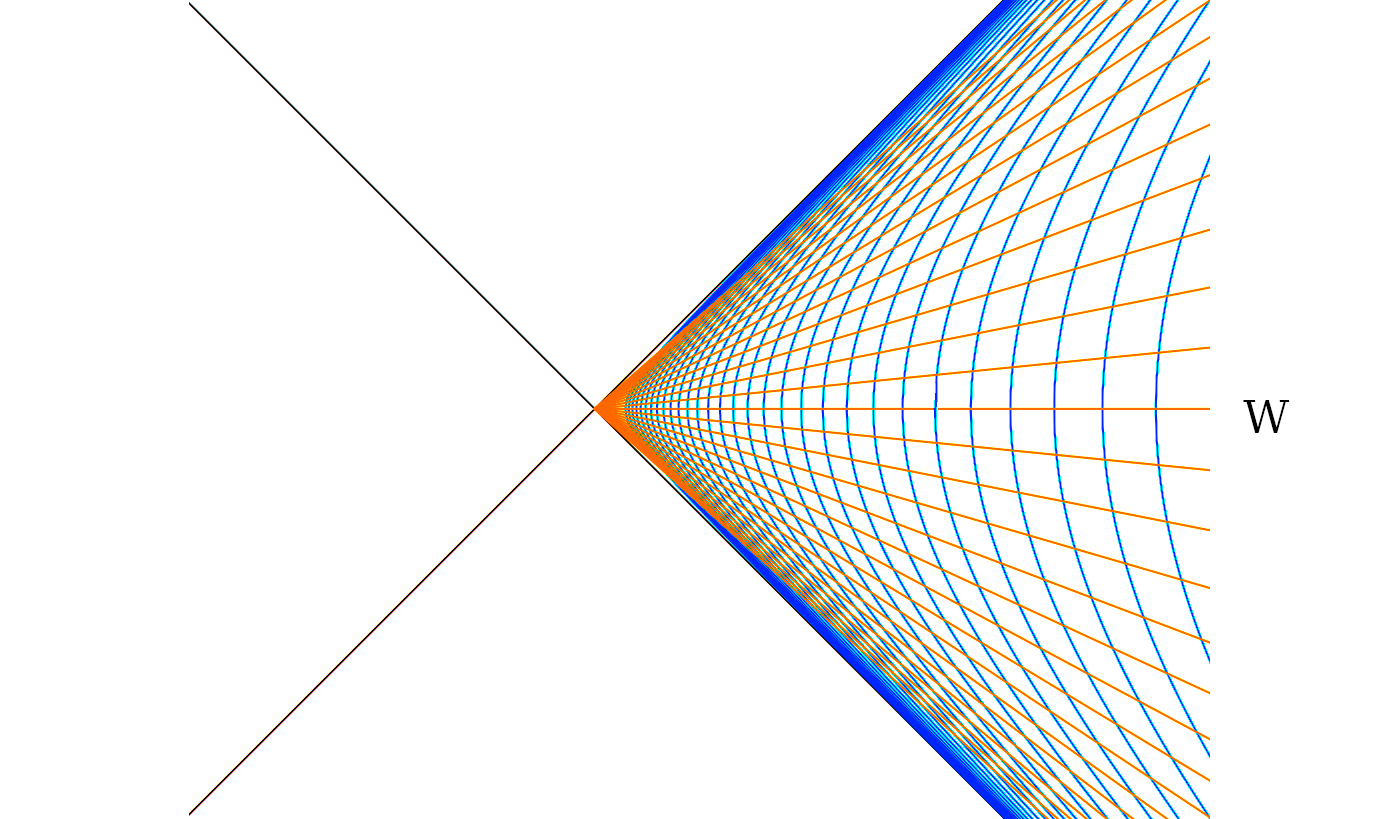
\includegraphics[scale=0.4]{rindler_w.png}
\caption{Rindler wedge $I$ on the right.}
\label{rindlerw}
\end{figure}

The massless Klein-Gordon equation in Rindler coordinates is
\begin{equation}
  \Box \phi = e^{-2a \xi}(-\partial_\eta^2 + \partial_\xi^2) \phi = 0
\end{equation}
which being the same form as equation (\ref{massless-wave-eq}), up to a conformal factor, has a basis of solutions with the same form as equation (\ref{amode})
\begin{equation}
 r_k(\eta,\xi) = \frac{1}{\sqrt{4 \pi \omega_k}} e^{-i(\omega_k \eta -k \xi)} + h.c.
\end{equation}
for each wave number $k$ and positive frequency $\omega_k = |k| > 0$.  These ``Rindler modes'' are in terms of $\eta$ and $\xi$ and are thus confined to the Rindler wedge $W$.  

\subsection{Unruh Modes}
For $\omega_k = k > 0$, and
\begin{equation}
  \begin{array}{lll}
    \alpha_k &= \frac{e^{\frac{\pi\omega_k}{2a}}}{\sqrt{2 \sinh \frac{\pi \omega_k}{a}}} &= \sqrt{\frac{1}{1 - e^{-2\pi\omega_k / a}}} \\
    \beta_k &= \frac{e^{\frac{-\pi\omega_k}{2a}}}{\sqrt{2 \sinh \frac{\pi \omega_k}{a}}} &= \sqrt{\frac{1}{e^{2\pi\omega_k / a} - 1}}, \\
  \end{array}
\end{equation}
noting that $\alpha_k^2 - \beta_k^2 = 1$. We analyticaly continue $r_k$, $r_{-k}$ to the $t,x$ plane as
\begin{equation}
  \begin{array}{ll}
    r_{+k} &= \frac{1}{\sqrt{4 \pi \omega_k}} e^{-i(\omega_k \eta - k \xi)} = \frac{1}{\sqrt{4 \pi \omega_k}} (a(-t + x + i \epsilon))^{\frac{i \omega_k}{a}} \\
    r_{-k} &= \frac{1}{\sqrt{4 \pi \omega_k}} e^{-i(\omega_k \eta + k \xi)} = \frac{1}{\sqrt{4 \pi \omega_k}} (a(-t - x + i \epsilon))^{\frac{-i \omega_k}{a}} \\
  \end{array}
\end{equation}
Define also
\begin{equation}
  \begin{array}{ll}
    \varphi_{+k} &= \frac{1}{\sqrt{4 \pi \omega_k}} e^{-i(\omega_k t - k x)}\\
    \varphi_{-k} &= \frac{1}{\sqrt{4 \pi \omega_k}} e^{-i(\omega_k t + k x)}\\
    \mu^R_k &= \alpha_k (r_k - r_{-k}^*) \\
    &= \frac{e^{\frac{\pi \omega_k}{2a}}}{\sqrt{2 \sinh \frac{\pi \omega_k}{a}}} \left(r_k - r_{-k}^* \right) \\
    &= \frac{1}{\sqrt{4 \pi \omega_k}\sqrt{2 \sinh \frac{\pi \omega_k}{a}}} \left( e^{\frac{\pi \omega_k}{2a}} \left(a(-t+x+i\epsilon)\right)^{\frac{i\omega_k}{a}} + e^{\frac{-\pi \omega_k}{2a}} \left(a(t+x-i\epsilon)\right)^{\frac{i\omega_k}{a}} \right) \\
    \mu^L_k &= \beta_k (r_k^* - r_{-k} )\\
    &=\frac{e^{\frac{-\pi \omega_k}{2a}}}{\sqrt{2 \sinh \frac{\pi \omega_k}{a}}} \left(r_k^* - r_{-k} \right) \\
    &=\frac{1}{\sqrt{4 \pi \omega_k}\sqrt{2 \sinh \frac{\pi \omega_k}{a}}} \left( e^{\frac{-\pi \omega_k}{2a}} \left(a(-t+x+i\epsilon)\right)^{\frac{-i\omega_k}{a}} + e^{\frac{\pi \omega_k}{2a}} \left(a(t+x-i\epsilon)\right)^{\frac{-i\omega_k}{a}} \right) \\
  \end{array}
\end{equation}
%TODO (verify U = r_k expressions)

\begin{figure}[h]
\centering
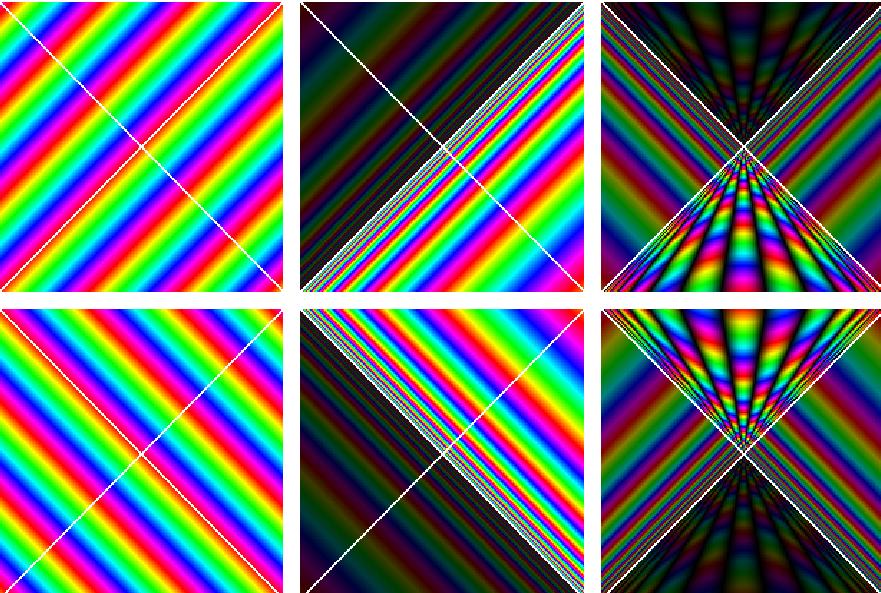
\includegraphics[scale=0.5]{unruh_mode_rainbow.png}
\caption{Space time diagrams for $\left[\begin{array}{ccc} \varphi_k & r_k & \mu^R_k \\ \varphi_{-k} & r_{-k} & \mu^L_k \end{array} \right]$.  Color is phase and brightness is magnitude. Rainbow order over time is consistent for $\varphi$ and $\mu$ since these are made up of positive frequency Minkowski modes. ($r_k$ is not consistent across the log branch.)}
\label{masslessshell}
\end{figure}

\subsection{Bogoliubov Transforms}
We have a Bogoliubov transformation matrix from $M$ to $W_0$ of
\begin{equation}
  \left[ \begin{array}{l}
    a^{(0)}_k \\
    a^{(0)}_{-k} \\
    \hline
    a^{(0)\dagger}_k \\
    a^{(0)\dagger}_{-k} \\
 \end{array} \right] = 
  \left[
\begin{array}{rr|rr}
    \alpha_k &       0   &  0       & \beta_k \\
    0        & -\alpha_k & -\beta_k & 0 \\
    \hline
    0        & \beta_k   & \alpha_k & 0 \\
    -\beta_k &    0      &   0      & -\alpha_k \\
\end{array} \right]_{k,q}
\left[ \begin{array}{l}
    c^R_q \\
    c^L_q \\
    \hline
    c^{R\dagger}_q \\
    c^{L\dagger}_q \\
 \end{array} \right]
\end{equation}
for a change of basis from $a^{(M)}$ to $c^R$ and $c^L$. 

We compute the Bogoliubov coefficients for
\begin{equation}
  \begin{array}{ll}
  a^{(c)}_k &= \int \dv{q} \alpha^{(cM)}_{kq} a^{M}_q + \beta^{(cM)}_{kq} a^{(M)\dagger}_q \\
  &= \int \dv{q} \alpha^{(c0)}_{kq} a^{(0)}_q + \beta^{(c0)}_{kq} a^{(0)\dagger}_q
  \end{array}
\end{equation}
as
\begin{equation}
  \begin{array}{ccl}
    \alpha^{(cM)}_{kq} &= \left<\varphi_q, r_k^{(c)} \right> &= \frac{1}{a \pi} \sqrt{\frac{\omega_k}{\omega_q}} \left(\frac{a}{q}\right)^{\frac{i\omega_k}{a}} e^{\frac{\pi \omega_k}{a}} \Gamma\left(\frac{i\omega_k}{a}\right) \\
    \beta^{(cM)}_{kq} &= \left<\varphi_q^*, r_k^{(c)} \right> &= \frac{1}{a \pi} \sqrt{\frac{\omega_k}{\omega_q}} \left(\frac{a}{q}\right)^{\frac{-i\omega_k}{a}} e^{\frac{-\pi \omega_k}{a}} \Gamma\left(\frac{-i\omega_k}{a}\right) \\
    \alpha^{(c0)}_{kq} &= \left<r_q^{(0)}, r_k^{(c)} \right> &= \frac{1}{2 \pi a}\sqrt{\frac{\omega_k}{\omega_q}} (ac)^{\frac{-i(\omega_q - \omega_k)}{a}} B\left(\frac{i\omega_k}{a}, \frac{i(\omega_q - \omega_k)}{a}\right) \\
    \beta^{(c0)}_{kq} &= \left<r_q^{(0)*}, r_k^{(c)} \right> &= \frac{1}{2 \pi a}\sqrt{\frac{\omega_k}{\omega_q}} (ac)^{\frac{-i(\omega_q + \omega_k)}{a}} B\left(\frac{-i\omega_k}{a}, \frac{i(\omega_q + \omega_k)}{a}\right) \\

  \end{array}
\end{equation}
We can compare absolute magnitudes for $M$ v.s. $W_c$ and see that they don't depend on $q$ or $c$
\begin{equation}
  \begin{array}{cc}
    \left|\beta_{kq}^{(c_1M)}\right|^2 = \left|\beta_{kq}^{(c_2M)}\right|^2 & \\
    \left|\beta_{kq}^{(c_1M)}\right|^2 = \left|\beta_{kq}^{(c_2M)}\right|^2 & \\
    \left|\beta_{kq}^{(cM)}\right|^2 / \left|\alpha_{kq}^{(cM)}\right|^2 = e^{\frac{-2\pi\omega_k}{a}}  & \text{   (thermal factor)} \\
 \end{array}
\end{equation}
The $c$ independence is expected since Unruh radiation is translation invariant. The $q$ independence can be strengthened as the expected number of particles in mode $k$
\begin{equation}
 \int \dv{q} \left|\beta_{kq}^{(cM)}\right|^2 = \frac{e^{\frac{-2 \pi \omega_k}{a}}}{2 \sinh \frac{\pi \omega_k}{a}} \int \dv{q} \frac{2}{a\pi |q|}
\end{equation}
where we factor out the divergent part to recover the radiation equation again.

We next turn to $W_c$ v.s. $W_0$ and also find $c$ independence there 
\begin{equation}
  \begin{array}{c}
    \left|\alpha_{kq}^{(0c_1)}\right| = \left|\alpha_{kq}^{(0c_2)}\right| \vspace{4pt}\\
    \left|\beta_{kq}^{(0c_1)}\right| = \left|\beta_{kq}^{(0c_2)}\right| \\
  \end{array}
\end{equation}
\begin{equation}
  \begin{array}{ll}
      \left|\beta_{kq}^{(0c)}\right|^2 / \left|\alpha_{kq}^{(0c)}\right|^2 \vspace{4pt} &= \left|\Gamma\left(\frac{i(\omega_q + \omega_a)}{a}\right)\right|^2 / \left|\Gamma\left(\frac{i(\omega_q - \omega_a)}{a}\right)\right|^2 \vspace{4pt} \\
  & = \frac{(\omega_q - \omega_k) \sinh \pi (\omega_q - \omega_k)}{(\omega_q + \omega_k) \sinh \pi (\omega_q + \omega_k)} \\
  \end{array}
  \label{nonzero_ratio}
\end{equation}
which is somewhat more surprising since this implies that $\int \dv{q} \left|\beta_{kq}^{(c_2c_1)}\right|^2$ is a $c_1$ and $c_2$ independent factor  for every shifted wedge inclusion.  In other words, the expected number of particles for a mode $r^{(c_2)}_k$ of $W_{c_2}$ in $W_{c_1}$'s vacuum is independent of the choice of shift $c_2$ and $c_1$.

More explicitly we have a transform matrix of $\Lambda_c$ from $W_0$ to $W_c$ 
\begin{equation}
  \left[ \begin{array}{l}
    a^{(c)}_k \\
    a^{(c)}_{-k} \\
    \hline
    a^{(c)\dagger}_k \\
    a^{(c)\dagger}_{-k} \\
 \end{array} \right] = \underbrace{
  \left[
\begin{array}{rr|rr}
    A_c        &       0   &  B_c            &  0 \\
    0        &      -A_c   &  0            & -B_c \\
    \hline
    \overline{B_c}        &    0      &  \overline{A_c} & 0 \\
    0 &    -\overline{B_c}      &   0           & -\overline{A_c} \\
\end{array} \right]_{k,q} }_{\Lambda_c}
  \left[ \begin{array}{l}
    a^{(0)}_q \\
    a^{(0)}_{-q} \\
    \hline
    a^{(0)\dagger}_q \\
    a^{(0)\dagger}_{-q} \\
 \end{array} \right]
\end{equation}
where $A_c = \alpha_{kq}^{(c0)} = P_c A_1 P_c^{-1}$  and $B_c = \beta_{kq}^{(c0)} = P_c B_1 P_c$ for a diagonal phase factor matrix
\begin{equation}
  P_c = P_{c,rs} = \delta(r - s) c^{\frac{i\omega_r}{a}} = e^{\frac{i H}{a} \log c}
\end{equation}
We can write $\Lambda_c$ out compactly out as
\begin{equation}
  \Lambda_c = Q_c \Lambda_1 Q_c^{-1}
\end{equation}
where
\begin{equation}
  Q_c = \left[\begin{array}{cccc}
        P_c, & 0 & 0 & 0 \\
        0 & P_c & 0 & 0 \\
        0 & 0 & P_c^{-1} & 0 \\
        0 & 0 & 0 & P_c^{-1} \\
    \end{array} \right] 
\end{equation}
Note that $\lim_{c\to 0} \Lambda_c = 1$ since the limit of $\lim_{c\to 0} \alpha_{kq}^{(c0)} = 1$ and $\lim_{c\to 0} \beta_{kq}^{(c0)} = 0$, which corresponds nicely to $\lim_{c\to 0} W_c = W_0$. The composition of Bogoliubov transforms, $\Lambda_{nc} = \Lambda_c^n$, yields
\begin{equation}
  \begin{array}{ll}    
    Q_{nc} \Lambda_1 Q_{nc}^{-1}  &= \Lambda_{nc} \\
         &= \left(Q_c \Lambda_{c} Q_c\right) \left( Q_c^{-1} \Lambda_{c} Q_c\right) \cdots \left(Q_c \Lambda_{c} Q_c\right) \\
  &= Q_c \Lambda_c^n Q_c^{-1} \\
  \end{array}
\end{equation}
so that
\begin{equation}
  \begin{array}{ll}
  \Lambda_c^n &= Q_c^{-1} Q_{nc} \Lambda_1 Q_{nc}^{-1} Q{c} \\
  &= Q_n \Lambda_1 Q_n^{-1}
  \end{array}
\end{equation}
and more generally we have a one parameter group given by
\begin{equation}
  \left\{\Lambda_0^x = Q_x \Lambda_0 Q_x^{-1} : x \in \mathbb{R} \right\}.
\end{equation}
This is an explicit version of modular flow, due to the von Neumann algebra modular automorphism associated with the translation $W_0 \rightarrow W_c$, studied in detail in Tomita-Takesaki theory \cite{Borchers2000}.  There we find thermal KMS states between open set inclusions in a much more general setting.


Consider a sequence
\begin{equation}
  W_{c_n} \subseteq \cdots \subseteq W_{c_i} \subseteq \cdots \subseteq W_{c_j} \subseteq W_{c_2} \subseteq W_{c_1}
\end{equation}
Then each $W_{c_i} \subseteq W_{c_j}$ involves particle production with a fixed squared magnitude for mode $k$.  We calculate this expected number of $W_{c_i}$ particles for mode $k$ in $W_{c_j}$'s vacuum
\begin{equation}
  \bra{0_{W_{c_j}}} a^{(c_i)\dagger}_k a^{(c_i)}_k \ket{0_{W_{c_j}}} = \frac{1}{2 \pi^2 k \sinh \frac{\pi k}{a}} \int_{x=0}^\infty \frac{x \sinh x}{(x+\frac{\pi k}{a}) \sinh(x+\frac{\pi k}{a})}
\end{equation}
which diverges.  The integrand goes to $e^{-\frac{\pi k}{a}}$ as $x$ gets large, so we can see that the expected number of particles in ratio goes to
\begin{equation}
  \frac{1}{m (e^{2m} + 1)} = \frac{1}{k (e^{\frac{2\pi \omega_k}{a}} - 1)}.
\end{equation}


\section{Appendix Formulas}
Some useful formula
\begin{equation}
  \int_{c}^\infty x^a (x-c)^b \dv{x} = c^{a+b+1} B(b+1, -a-b-1)
\end{equation}
TODO, check this next one
\begin{equation}
  \int_{-\infty}^\infty e^{ikx} x^b \dv{x} = -\frac{2i}{k^{b+1}} e^{\frac{-\pi b}{2}} \Gamma(b+1)
\end{equation}
This is useful for the shifted wedge inner products. Let
\begin{equation}
  f_{k,b,d} = \left(a\left(b(t-i\epsilon)+x\right)\right)^\frac{id\omega_k}{a}
\end{equation}
Then
\begin{equation}
  \left< f_{k,b_k,d_k}, f_{q,d_q,d_q}\right> = \frac{1}{2\pi} \sqrt{\frac{\omega_k}{\omega_q}} (ac)^\frac{i(d_k\omega_k - d_q \omega_q)}{a} \left((-d_k)\frac{b_k + b_q}{2} \right) B\left(\frac{id_k\omega_k}{a}, \frac{-i(d_k\omega_k - d_q \omega_q)}{a}\right)
\end{equation}
We frequently use
\begin{equation}
  |\Gamma(ib)|^2 = \frac{\pi}{b \sinh \pi b}
\end{equation}


\section{Driving Sources}

THE REST OF THIS NEEDS WORK

We can ask {\bf ``What exactly is accelerating the observer?''}.  So far we have not tried to answer this question.  In our ignorance, we have recovered, in the math, that something thermal is going on in terms of particle creation.  More specifically, Figure \ref{analytic} depicts the situation where a Rindler mode $r_k$ is either a left moving {\bf emission} from the Rindler observer or a right moving {\bf absorption} by the Rindler observer.  We will next provide an answer to this question, using a driving source to capture the thrust. Then we will see that the radiation term shifts away, back into the source field.  The math is the same, but the interpretation will change.


%%%%%%%%%%%%%%%%%%
BREAK BREAK BREAK
%%%%%%%%%%%%%%%%%%


To that end, consider a driving source field $J$ in the sense of Schwinger \cite{schwinger} 

\begin{equation}
  J(k) = c_{-k}^{(2)\dagger} \frac{e^\frac{-\pi \omega_k}{2a}}{\sqrt{2 \sinh \frac{\pi \omega_k}{a}}} r_k(x,t) \theta(T - t) \theta(T+t)
\end{equation}
using an extended Rindler mode $r_k$.  It is active for some finite amount of time $-T \le t \le T$ and is crafted to exactly compensate for the cross term in equation (\ref{bogo}) as we aim to see.  The form of $J$ is invariant under right or left shift as functions of $u$ or $v$ so that the Klein Gordon dot product will be invariant also.

We add the source term to the Lagrangian

\begin{equation}
\mathscr{L} = -\frac{1}{2} \eta^{\mu\nu}\partial_\mu \phi \partial_\nu \phi - J\phi
\end{equation}
The Euler-Lagrange equation leads to an inhomogeneous Klein-Gordon equation
\begin{equation}
  \Box  \phi = J
\end{equation}
%Consider the retarded Green's function $G_R$, as in \cite{beisert} for instance, in momentum space
%\begin{equation}
%  G_R(k) = 1 / k^2 ???
%\end{equation}
Let $a_k = a_k^{in}$ be the annihilation operator for $t<-T$ and let $a_k^{(out)}$ be the annihilation operator for time $t > T$.  Then one can find using the retarded Green's function, as in \cite{beisert} for instance, that $a_k^{out} = a_k^{in} + i J(k)$.



%%%%%%%%%%%%%%%%%%
BREAK BREAK BREAK
%%%%%%%%%%%%%%%%%%


Consider these multiples of Rindler modes on the entire $(t,x)$-plane
\begin{equation}
f_k(u) = \frac{e^{\frac{\pi \omega_k}{2a}} {(au)}^{\frac{i\omega_k}{a}}}{ \sqrt{2\sinh\left(\frac{\pi\omega_k}{a}\right)}}
\end{equation}
\begin{equation}
g_k(v) = \frac{e^{\frac{\pi \omega_k}{2a}} {(av)}^{\frac{i\omega_k}{a}}}{ \sqrt{2\sinh\left(\frac{\pi\omega_k}{a}\right)} }
\end{equation}
Let $\phi$ be a free scalar field in the flat $1+1$ dimensional Minkowski spacetime.  We will consider $f_k(u)$ and $g_k(v)$ as driving sources
\begin{equation}
\label{ab}
\rho(u,v) = \alpha f_k(u) + \beta g_k(v).
\end{equation}
with non-negative real convex combination $\alpha + \beta = 1$. The drivers $f_k$ and $g_k$ are functions of $u$, the future $I$-horizon and of $v$, the past $I$-horizon respectively.  Both generate excitations, which we identify with emission and absorption thrusts respectively.


The sources can originate from a coupling term, $\rho \phi$, added to the free scalar Lagrangian.  We also add in a $i \epsilon$ term so that our integrals converge.
\begin{equation}
\mathscr{L} = -\frac{1}{2} \partial^\mu \phi \partial_\mu \phi + \rho\phi + \frac{i \epsilon}{2}  \phi^2
\end{equation}
The Euler-Lagrange equation leads to an inhomogeneous Klein-Gordon equation
\begin{equation}
  \Box  \phi = \rho + i \epsilon \phi
\end{equation}
as presented in \cite{beisert}.  In \cite{beisert} it is assumed that the source is only active for a finite amount of time.  We let $\rho$ be active for all time.  The argument in \cite{beisert} seems to be adaptable to $\rho$.

We will want to integrate $\rho$ on shell in momentum space, which for a massless source is the positive energy part of the massless shell.  The two positive energy ``horizons'' border $p_u \le 0$ and $p_v \le 0$, see Figure \ref{masslessshell}.  Proceeding to take the Fourier transform of the function $f_k(u)$.  WLOG since $g_k(v)$ is of the same form.  We will continue to assume that $\omega_k$ and $a$ are positive. Define the kernel

\begin{equation}
  A = e^{-i p_u u} (au)^\frac{i\omega_k}{a} du
\end{equation}
and then we have
\begin{equation}
\label{finalnorm}
  \hat{f_k}(p_u) =  \frac{e^{\frac{\pi \omega_k}{2a}}}{\sqrt{2 \sinh \left({\frac{\pi\omega_k}{a}}\right)}}  \int_{-\infty}^\infty A
\end{equation}
where $L=\int_{-\infty}^0 A$ and $R=\int_0^\infty A$ are the left and right sides of the total integral $L + R$.

\begin{figure}[h]
\centering
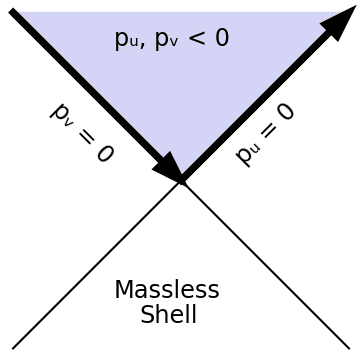
\includegraphics[scale=0.5]{massless_shell.png}
\caption{Massless shell is when $p_u$ = $p_v$ = 0}
\label{masslessshell}
\end{figure}

\begin{figure}[h]
\centering
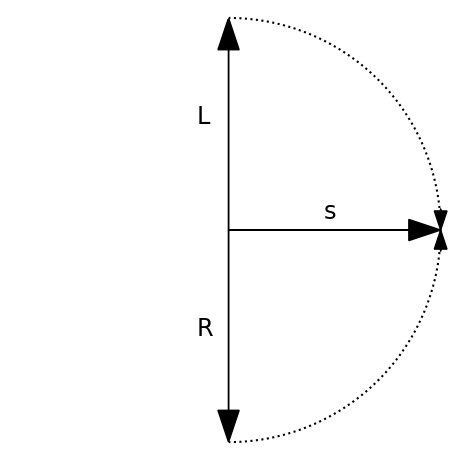
\includegraphics[scale=0.3]{contour.png}
\caption{Using contours with large radius we convert the $L$ integral that goes to $i\infty$, and the $R$ integral that goes to $-i\infty$, to integrals with $s$ going to real $\infty$.}
\label{fig:x cubed graph}
\end{figure}

We rewrite the integrals using a complex changes of variables, $s$ = $ip_uu$, and contour integrals.
The $L$ integral for real $p_u<0$ is
\begin{equation}
\begin{split}
  L(p_u) & = -\int_0^{i\infty} e^{-s}\left(\frac{ias}{-p_u}\right)^\frac{i\omega_k}{a} \left(\frac{i}{-p_u}\right)ds \\
  & = \frac{-i}{a} \left(\frac{a}{-p_u}\right)^{\frac{i\omega_k}{a} + 1} \int_0^\infty \left(is\right) ^ \frac{i\omega_k}{a} e^{-s} ds \\
  & = \frac{-i}{a} \left(\frac{a}{-p_u}\right)^{\frac{i\omega_k}{a} + 1} \Gamma\left(\frac{i\omega_k}{a} + 1\right) e^{-\frac{\pi \omega_k}{2a}} \\
  & = \frac{1}{2} \Gamma\left(\frac{i\omega_k}{a} + 1\right) e^{-\frac{\pi \omega_k}{2a}} B(p_u)\\
\end{split}
\end{equation}
where
\begin{equation}
B(p_u) = \frac{-2i}{a} \left(\frac{a}{-p_u}\right)^{\frac{i\omega_k}{a} + 1} 
\end{equation}
The change of $i\infty$ to $\infty$ is made by using a large radius contour which rotates the endpoint 90 degrees clockwise.  The term $e^{-s}$ goes to zero around the large radius circle.

The same calculation for $R$ is done using a counter-clockwise contour this time.
\begin{equation}
\begin{split}
  R(p_u) = \frac{1}{2}\Gamma\left(\frac{i\omega_k}{a} + 1\right) e^{-\frac{\pi \omega_k}{2a}} B(p_u)
\end{split}
\end{equation}

We get back to $f_k(u)$ and apply the normalization from equation (\ref{finalnorm})
\begin{equation}
\widehat{f_k}(p_u) = \frac{e^{\frac{\pi \omega_k}{2a}}}{\sqrt{2 \sinh \left({\frac{\pi\omega_k}{a}}\right)}}  ( L(p_u) + R(p_u) )
\end{equation}
So
\begin{equation}
\label{fourier}
\begin{split}
\widehat{f_k}(p_u) & = \frac{\Gamma\left(\frac{i\omega_k}{a} + 1\right)}{\sqrt{2 \sinh \left({\frac{\pi\omega_k}{a}}\right)}} B(p_u)\\
\widehat{g_k}(p_v) &= \frac{\Gamma\left(\frac{i\omega_k}{a} + 1\right)}{\sqrt{2 \sinh \left({\frac{\pi\omega_k}{a}}\right)}} B(p_v)
\end{split}
\end{equation}
\section{Interpretation}
The driving source $\rho$, with mixed absorption and emission thrusts $\alpha$ + $\beta$ = 1, contribute excitations to the scalar field $\phi$. Equations (\ref{ab}) and (\ref{fourier}) let us write down the expected change of energy
\begin{equation}  
  \label{number}
  \begin{split}
    \mathbb{E}[\Delta E] &= \frac{1}{4\pi} \int{|\rho(p)|^2 dp} \\
    &= \frac{\alpha}{4\pi} \int{\left|\widehat{f_k}(p_u)\right|^2 dp_u} + \frac{\beta}{4\pi}\int{\left|\widehat{g_k}(p_v)\right|^2dp_v} \\
    &= \frac{\left|\Gamma\left(\frac{i\omega_k}{a} + 1\right)\right|^2}{2 \sinh \left({\frac{\pi\omega_k}{a}}\right)} \frac{1}{4\pi} \int{{\left|B(p)\right|^2} dp} \\
    &=  \frac{\left|\Gamma\left(\frac{i\omega_k}{a} + 1\right)\right|^2}{2 \pi a \sinh \left({\frac{\pi\omega_k}{a}}\right)} \int{a/|p|^2 dp}\\  
&=I(\omega_k) P
  \end{split}
\end{equation}
where the integrals are on the positive energy massless shell with contributions from $p_u$ on the left piece and $p_v$ on the right piece.  We factored out $P = \int{a/|p|^2}$ with a remaining $p$ independent positive real coefficient $I(\omega_k)$.

Without being more careful we end up with inferred problems --- The integrals do not converge at zero, where $P$ explodes.  But this infinity cancels when we compare the spectral radiances to each other, $I(\omega_{k_1}) / I(\omega_{k_2})$.

The magnitude of our Gamma function has known asymptotics \cite[Eq.~5.11.9]{NIST:DLMF}
\begin{equation}
\left|\Gamma\left(\frac{i\omega_k}{a} + 1\right) \right|^2 \sim \left(\frac{2 \pi \omega_k} {a}\right) e^{-\frac{\pi\omega_k}{a}}
\end{equation}
Plugging this into equation (\ref{number}) we find the average energy of the mode, the $1+1$ dimensional Planck distribution function, and thus recover the Unruh's radiation spectrum from a thrust driven field.
\begin{equation}
\frac{1}{P} \mathbb{E}[\Delta E] = I(\omega_k) \sim \frac{\omega_k}{e^{\frac{2 \pi \omega_k}{a}}-1}
\end{equation}
Compare this to equation (\ref{radeq}) and references \cite{unruh} and \cite{Frodden}.

\begin{figure}[h]
\centering
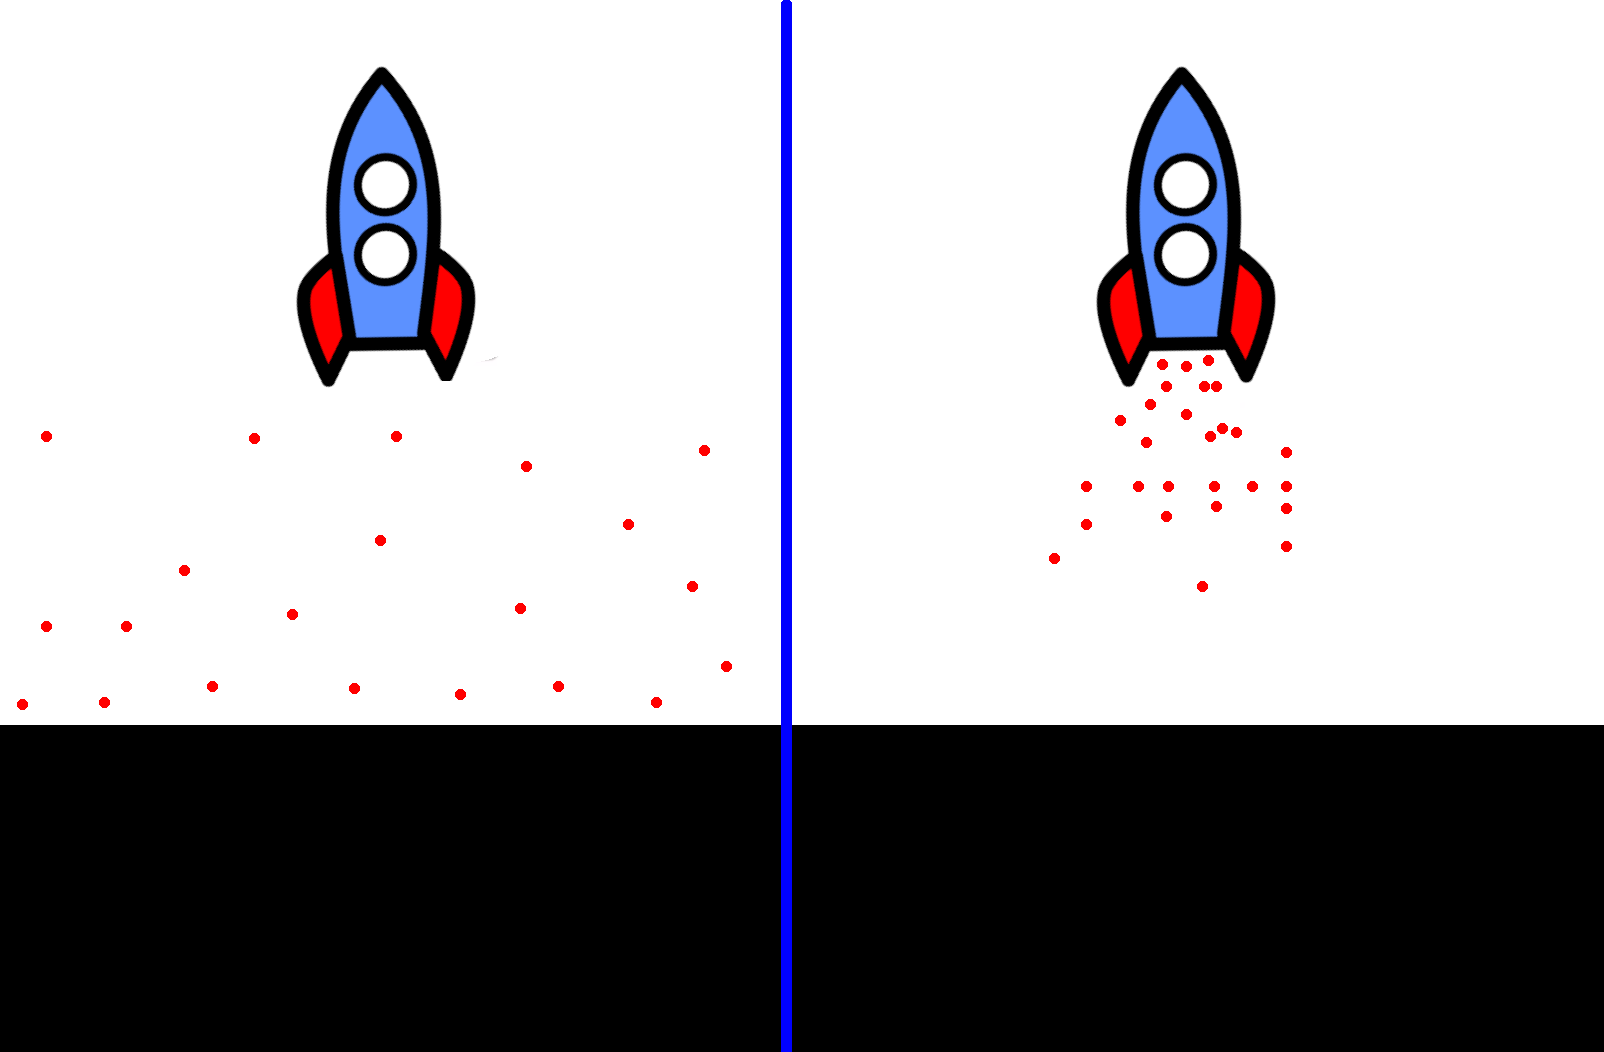
\includegraphics[scale=0.5]{rocket_inertial.png}
\caption{Unruh picture of an event horizon radiating in accelerating frame radiating on the left. Our picture of a rocket under inertial acceleration thrusting on the right.}
\label{rocket_inertial}
\end{figure}

\section{Other Types of Driving Sources}
TODO
\section{Ricci Scalar as a Driving Source}
TODO
\section{Fields with Interaction}
TODO

\section{Conclusion and Prediction}
If the thrust required to accelerate a detector is not explicitly accounted for, it manifests instead as an apparent thermal feature of the vacuum—Unruh radiation. However, as demonstrated in this paper, Unruh radiation can be directly explained as a consequence of thrust. This perspective leads to the prediction that neither Unruh radiation nor Hawking-Bekenstein radiation should appear independently of the thrust that drives the system.

\begin{figure}[h]
\centering
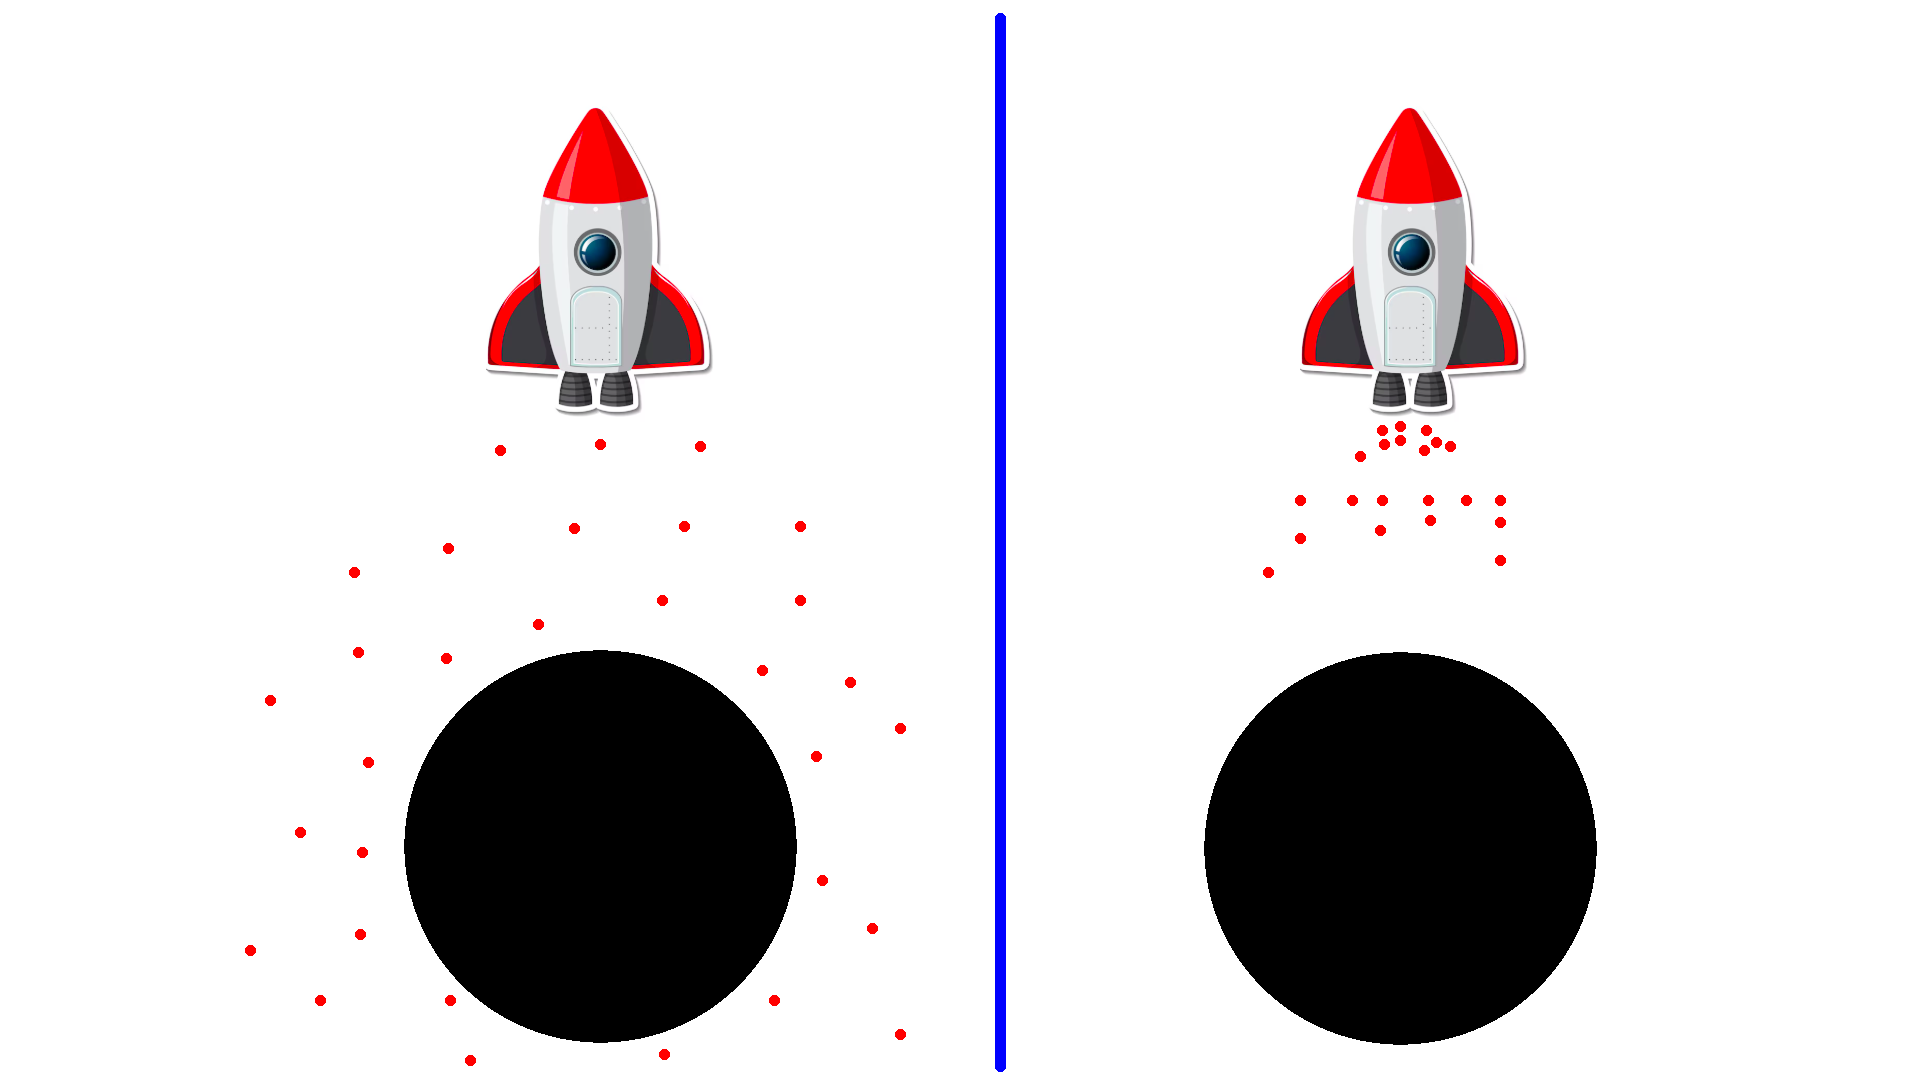
\includegraphics[scale=0.5]{rocket.png}
\caption{Hawking picture of black hole radiating on the left. Our picture of a rocket thrusting on the right.}
\label{rocket}
\end{figure}

\section{Acknowledgments}
Thanks to Ben Commeau and Daniel Justice for useful discussions.

\bibliographystyle{ieeetr}
\bibliography{bibliography}

\end{document}
